\chapter{Lösungsidee}

\textbf{Das Spieldesign}

Das CZGame sollte sich stark am realen Leben orientieren. Schulgebäude und zugehörige Accessoires sollten im Rahmen der Umsetzungsmöglichkeiten und der Spielidee eine größtmögliche Realitätstreue behalten und dem Carl-Zeiss-Gymnasium in Jena nachempfunden sein (siehe Abbildung \ref{abb:01beispiel} und \ref{abb:02beispiel}) .


Da das Spiel im Pixelartdesign entstehen sollte, musste ein geeignetes Programm genutzt werden um das Format der Graphik digital und in Pixeln zu implementieren. Das herkömmliche Format eines Computerbildschirms beträgt standardmäßig 16 zu 9. Da das CZGame als PC-Spiel entworfen werden sollte wurde ein rechteckiges Format der Größe 240 zu 135 Pixeln gewählt, das diesem Verhältnis entspricht.


Als Programm wurde das kostenlose und qualitativ hochwertige Onlinetool \emph{Pixelart} verwendet. 
Innerhalb der Gruppe \emph{Graphikdesign} wurde die Arbeit zum erstellen der Hintergrundgraphiken aufgeteilt. Durch die kollektive Zusammenarbeit beim erstellen der Bilder, kommt es im Endergebnis zu einer großen Vielfalt an Farben und Formen, die die Freude am Spiel fördern sollen. Da jeder die Möglichkeit hatte selbst schulspezifische Mottos in die Hintergründe einzubringen, sorgt jeder Raum ganz individuell für eine Überraschung.
\begin{figure}[ht]
 \centering
 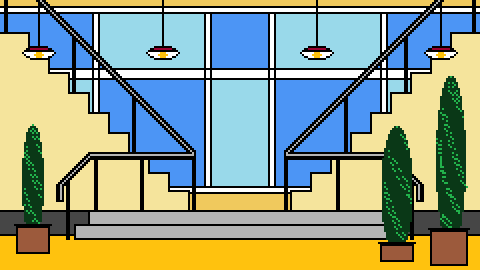
\includegraphics[scale=0.5]{bilder/Foyer.png}
 \caption{Das Foyer bildet den Ausgangsort des CZGames}
 \label{abb:01beispiel}
\end{figure}

Die Gruppe \emph{Graphikdesign} stand während den Arbeiten an den Bilddateien in starkem Austausch mit der Gruppe \emph{Item- \& Charakterdesign} so wie mit den Verantwortlichen für das Erstellen von Minigames. Unter anderem musste das Größenverhältnis der Charaktere und Spielerfiguren auf die Größe der Räume angepasst werden. 

Für das Design der einzelnen Spielerfiguren und der Figuren des Lehrkörpers wurde aufgrund der guten Kompatibilität einzelner Bilddateien untereinander ebenfalls \emph{Pixelart} verwendet. So konnte später in der Java-Implementierung ermöglicht werden, das zu Beginn des Spiels jeder Spieler seine individuelle Spielerfigur erstellen kann, dies erhöht das eigene Spielvergnügen und gibt dem Spiel eine persönliche Note.



\begin{figure}[ht]
 \centering
 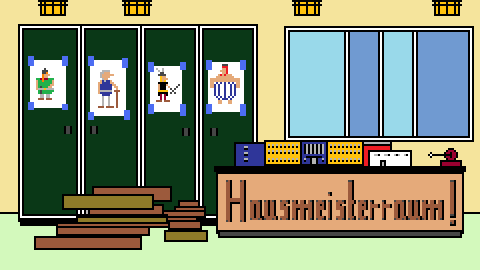
\includegraphics[scale=0.5]{bilder/Hausmeisteraum.png}
 \caption{Im Raum des Hausmeisters ist ein Modell der Schule zusehen}
 \label{abb:02beispiel}
\end{figure}

\textbf{Der Spielaufbau}

Das CZGame sollte grundsätzlich die Form eines Point-and-Click-Spiels erhalten. Während der Spieler sich über dafür vorgesehene Pfeile durch das Schulgebäude bewegt, sollte die Möglichkeit eines sogenannten Minigames oder einer Challenge, ähnlich einer mündlichen Prüfung mit einem Mitglied des Lehrkörpers, bestehen. Das Wechseln der Räume erfolgt über Standbilder, in denen die Figur durch 

Die Minigames wurden von einem eigens dafür bestimmten Team entworfen und in Java implementiert. 
Dabei sollte in jedem der folgenden Fächer die Möglichkeit eines Minigames und einer mündlichen Prüfung bestehen:
\begin{itemize}
    \item Fachschaft Biologie
        \begin{itemize}
        \item Das Minigame der Fachschaft Biologie ähnelt in seine Grundzügen dem Pflanzentestat am Carl-Zeiss-Gymansium Jena. Um eine möglichste Originaltreue der zuerkennenden Pflanzen zu schaffen wurden über 30 Pflanzen als erkennbare Graphik gepixelt und in Java implementiert.
        \end{itemize}
    \item Fachschaft Chemie
        \begin{itemize}
        \item Das Chemie Minigame entspricht der bekannten Form eines Water-Sort-Puzzles.
        \end{itemize}
    \item Fachschaft Informatik
        \begin{itemize}
        \item In der Fachschaft Informatik wird zum Lösen des Minigames Kenntnis von Grundlegenden informatischen Schaltarten vorausgesetzt. Da hier auf der Basis von Schaltungen auf das entsprechende Schaltzeichen zurück geschlossen werden muss.
        \end{itemize}
    \item Fachschaft Mathematik
        \begin{itemize}
        \item Das Lösen von Tangramfiguren der Hauptteil der Mathematikminigames.
        \end{itemize}
    \item Fachschaft Physik
        \begin{itemize}
        \item Um einen Ball auf eine vorgegebene Stelle zu positionieren muss im Minigame der Fachschaft Physik der Zusammenhang von Kräften und deren Vektoren erkannt und angewendet werden. 
        \end{itemize}
\end{itemize}

Jedes Minigame sollte zudem aus drei unterschiedlichen Leveln bestehen, mit einem aufsteigenden Schwierigkeitsgrad von Eins bis Drei. Beim erfolgreichen Lösen eines solchen Levels, gewinnt der Spieler Items, die sich als Symbole für die zuvor genannten Fachschaften herausstellen.

Alle Items sind gleichwertig und können als unterstützendes Mittel während einer mündlichen Prüfung in jedem Fach eingesetzt werden. Das Sammeln der Items sowie der Einsatz erfolgt automatisch oder über dafür vorgesehene Buttons.


In der gesamten Arbeit soll auf Abbildungen verwiesen werden (siehe Abbildung \ref{abb:beispiel}) und gegebenenfalls hilfreiche Zitate eingefügt werden.\newline
Wörtliche Rede wird in Latex zwischen \verb|"`| und \verb|"'| gesetzt. 

\begin{quote}
 "`\blindtext"'\footnote{Heinemann, 1998, S.\,280}
\end{quote}
